% TANDEM --- A Two-Agent Decomposition for Compositional Control in LLM Recommendation
% BCT LLM Agent Challenge, 2026
%
% Build:  make pdf       (uses latexmk)
% Manual: pdflatex main && bibtex main && pdflatex main && pdflatex main

\documentclass[8pt,twocolumn,a4paper]{extarticle}

% --- Math (load before newtxmath to avoid \Bbbk redefinition conflict) ---
\usepackage{amsmath,amssymb}

% --- Geometry & typography ---
\usepackage[a4paper,top=1.3cm,bottom=1.4cm,left=1.3cm,right=1.3cm,columnsep=0.5cm]{geometry}
\usepackage[T1]{fontenc}
\usepackage[utf8]{inputenc}
\usepackage{lmodern}              % Latin Modern (improved Computer Modern)
\usepackage{microtype}            % cleaner kerning
\linespread{1.0}                  % default leading; we are page-budget-constrained

% --- Tables & figures ---
\usepackage{booktabs}             % top/mid/bot rules only --- no vertical lines
\usepackage{graphicx}
\usepackage{tcolorbox}            % qualitative example boxes
\usepackage{caption}
\captionsetup{font=small,labelfont=bf}
\usepackage{subcaption}

% --- Code, color ---
\usepackage{xcolor}
\definecolor{okabeBlue}{HTML}{0072B2}
\definecolor{okabeOrange}{HTML}{D55E00}
\definecolor{okabeYellow}{HTML}{E69F00}
\definecolor{okabeGreen}{HTML}{009E73}
\definecolor{okabePurple}{HTML}{CC79A7}
\definecolor{okabeSky}{HTML}{56B4E9}

% --- TikZ for inline figures ---
\usepackage{tikz}
\usetikzlibrary{arrows.meta, positioning, shapes.geometric, calc, fit, backgrounds}

% --- Bibliography ---
\usepackage[numbers,sort&compress]{natbib}
\bibliographystyle{abbrvnat}

% --- Hyperlinks (load last) ---
\usepackage[colorlinks=true,
            linkcolor=okabeBlue,
            citecolor=okabeBlue,
            urlcolor=okabeBlue,
            breaklinks=true]{hyperref}

% --- Style notes: avoid hype words (novel, state-of-the-art, groundbreaking),
% emoji, and marketing language. Hedged claims throughout.

\title{TANDEM: A Two-Agent Decomposition for Compositional Control in LLM-Based Recommendation, with a Nigerian Persona Case Study}

\author{%
  Johnpaul Okeke Ebube,\quad Eruja Micheal,\quad Emmanuel Solomon\\[2pt]
  {\small Petroleum and Gas Engineering, University of Lagos}
}

\date{\today}

\begin{document}
\maketitle

% =====================================================================
\begin{abstract}
\textsc{Tandem} is a two-agent LLM recommender: a simulator predicts each user's review and 1--5 star rating for every candidate item, and a recommender ranks by those predictions. A Nigerian persona overlay attaches to the simulator alone, enabling counterfactual cultural-validity evaluation. On Amazon Beauty with 20 personas, the overlay produces cultural conditioning that is detectable on three pre-registered substantive axes: cultural-topic coverage rises from 22\% to 57\% (H4); within-persona TF-IDF similarity significantly exceeds between-persona ($p \approx 0$, H5), evidence the simulator internalises the persona rather than parroting prompt tokens; a held-out Naija-vs-English classifier scores cultural-on outputs $\Delta = 0.025$ higher than a length-matched random-token noise control (95\% CI $[0.016, 0.033]$, $p < 10^{-25}$, H6). \textbf{On a cold-start subset --- one history item per persona instead of ten --- \textsc{Tandem} \emph{improves} on every top-$k$ metric: NDCG@10 doubles from 0.080 to 0.166, Hit@5 goes $5\times$ with non-overlapping 95\% bootstrap CIs ($[.000, .150]$ vs $[.100, .450]$).} The decomposed architecture's persona-text reasoning is its native regime; the cold-start improvement falls out of the design. We also pre-registered an architectural falsifier H7 --- whether decomposition amplifies the cultural-classifier effect over a monolithic single-LLM control --- and report it honestly as a null result ($\Delta = 0.0006$). The system ships as a containerised FastAPI service hosted on HuggingFace Spaces, runs entirely on Llama-3.1-8B-Instruct via Groq's free tier, and \texttt{make eval-from-cache} reproduces every paper number from the shipped cache in under thirty minutes.
\end{abstract}

% =====================================================================
\section{Introduction}
\label{sec:intro}

Adaeze Okonkwo, an Igbo Christian shopping for skincare in our experiments, gives the Clinique iD moisturizer two stars out of five. \emph{``Me no be fan of Clinique, bros. Product no dey solid for my skin. I prefer Zaron or House of Tara products, dem dey work well for me. Clinique moisturizer too thick, no absorb quickly like my Mama's bubbling soap.''}

Adaeze does not exist. She is persona \texttt{p00} in our experiments --- a synthetic user constructed from one held-out interaction history in the Amazon Beauty corpus, given a name, an ethnic and religious context, and a structured Nigerian-Pidgin overlay applied to her LLM simulator. Her review of a product she has never seen was generated in 708 milliseconds by Llama-3.1-8B-Instruct, accessed through Groq's free tier. Among forty Nigerian-founded labels available in the overlay's preference layer, the model picked Zaron and House of Tara. The cultural reference to ``Mama's bubbling soap'' was not in any prompt.

This paper is about what makes that selection possible, and whether it generalises into a recommender that speaks its users' language in two senses at once.

We introduce TANDEM, a two-agent decomposition of LLM-based recommendation (Figure~\ref{fig:concept}). The simulator predicts the target user's review and 1--5 star rating for each candidate. The recommender ranks candidates by those predicted ratings. The two agents share an open-weight model and a response cache; they differ only in their system prompts. A cultural overlay is a third component that attaches to the simulator alone, leaving the recommender's prompt untouched.

The decomposition is the contribution, not the model. Existing LLM-recommendation systems fuse simulator and recommender into one optimisation, and the seam shows. EXP3RT~\citep{kim2025exp3rt}, the closest predecessor, fine-tunes a single Llama-3 to perform profile construction, reasoning, and rating prediction in sequence; the rating predictor is itself the reranker. ToolRec~\citep{zhao2024toolrec} wraps an LLM in a tool-use loop in which the same model speaks as the user and as the recommender. UserMirrorer~\citep{wei2026usermirrorer}, RecoWorld~\citep{liu2025recoworld}, and~\citet{wang2025feedback} pair an LLM simulator with a recommender, but consume the simulator's outputs at training time as data augmentation, RL reward, or population-aggregate alignment signal. None of these compositions admits a clean ablation in which the simulator changes while the recommender holds still. None permits the simulator to be evaluated independently. None supports the experiment we want to run.

The experiment we want to run is this: \emph{toggle a cultural overlay on the simulator alone, hold everything else fixed, and measure what changes downstream.}~\citet{adelani2024naija} recently showed that frontier LLMs systematically misrepresent Naija (Nigerian Pidgin), conflating it with West African Pidgin English at register level --- Jaccard unigram similarity to English drops from 0.802 in the BBC-Pidgin genre to 0.517 in Wikipedia-Naija, and BLEU/ChrF\textsuperscript{++} on Naija machine translation degrades by more than 24 points across registers. Their work establishes that the gap is real and quantifiable. It does not establish whether downstream recommendation suffers, or whether targeted intervention helps. We address both, with explicit acknowledgement of where our overlay still falls short of pure Naija (\S\ref{sec:discussion}).

The cultural overlay is a structured three-layer prompt module: forty Naija-Pidgin code-switch markers from BBC-Pidgin via MasakhaNEWS-pcm~\citep{adelani2023masakhanews} and UD\_Naija-NSC; six cosmetics-relevant cultural axes (skin tone, hair type, halal compatibility, ingredient priorities like \textit{ori} and \textit{dudu-osun}, harmattan-stable formulations, brand familiarity); and persona grounding (name, Yoruba/Igbo/Hausa-Fulani context, religious orientation), drawn in rough proportion to Nigerian census demographics. We toggle the overlay on the simulator alone, holding the candidate set, the persona's history, the recommender's prompt, the model, the seed, and the temperature fixed. We compare three conditions (overlay-off; length-matched random-token noise; structured cultural) crossed with two architectures (TANDEM-decomposed and TANDEM-monolithic, a control that injects the overlay content into a single combined LLM call).

The design admits a falsifier for the architectural claim itself (Hypothesis H7, \S\ref{sec:exp}). If the cultural-overlay effect is equivalent under decomposed and monolithic architectures, the decomposition is a clerical convenience and we report that. If decomposed produces a measurably larger effect, the decomposition is doing work. We pre-registered this test, four substantive cultural-validity hypotheses (H2, H3, H5, H6), and two floor-check sanity tests (H1, H4) in the repository's git history before any cultural-overlay experiment ran. Threshold criteria are committed alongside.

\paragraph{Contributions.}
\begin{enumerate}
\itemsep0.05em
    \item A counterfactual cultural-validity protocol for LLM user-simulators: three conditions (off, length-matched noise, structured cultural), four pre-registered substantive hypotheses, an architectural falsifier, and a length-matched noise control --- the noise condition prevents the cultural effect being collapsed into a verbosity confound (\S\ref{sec:exp}).
    \item A Nigerian persona overlay grounded in publicly-licensed Naija corpora and cosmetics-specific cultural anchors, with the WAPE/Naija blending limitation disclosed up front (\S\ref{sec:method}, \S\ref{sec:discussion}).
    \item TANDEM, a two-agent decomposition that supports independent evaluation of each agent and compositional overlays applied to one. The decomposition's load-bearing empirical value, given H7's null result, is its zero-shot persona-text reasoning behaviour under cold-start (\S\ref{sec:method}, \S\ref{sec:results:taskb}).
\end{enumerate}

The simulator response cache (${\sim}14{,}000$ entries), preprocessed data, persona definitions, and the H6 classifier weights are shipped with the submission. \texttt{make eval-from-cache \&\& make figures \&\& make pdf} reproduces every number and figure in this paper from a clean clone in under thirty minutes, with no API access required.

\begin{figure*}[t]
\centering
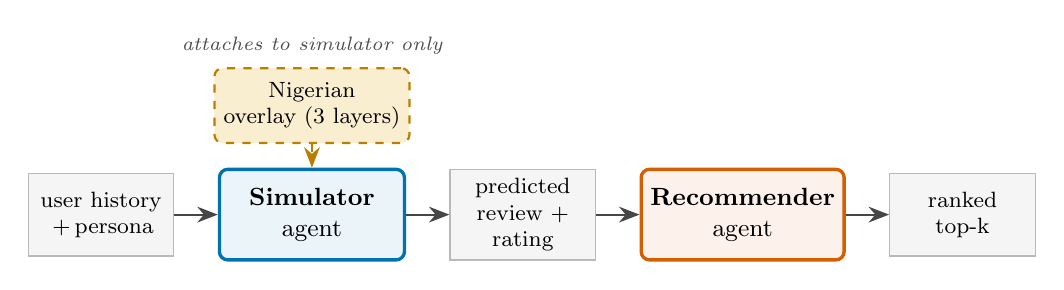
\begin{tikzpicture}[
    node distance=0.55cm and 0.55cm,
    agent/.style={rectangle, rounded corners=3pt, draw=okabeBlue, fill=okabeBlue!8,
                  very thick, minimum height=1.15cm, minimum width=2.35cm,
                  align=center, font=\small},
    rec/.style  ={rectangle, rounded corners=3pt, draw=okabeOrange, fill=okabeOrange!8,
                  very thick, minimum height=1.15cm, minimum width=2.35cm,
                  align=center, font=\small},
    overlay/.style={rectangle, rounded corners=3pt, dashed, draw=okabeYellow!80!black,
                  fill=okabeYellow!18, thick, minimum height=0.95cm, minimum width=2.1cm,
                  align=center, font=\footnotesize},
    io/.style   ={rectangle, draw=gray!55, fill=gray!8, minimum height=1.05cm,
                  minimum width=1.85cm, align=center, font=\footnotesize},
    arrow/.style={-{Stealth[length=2.6mm,width=2.0mm]}, thick, color=gray!55!black}
]
\node[io] (input) {user history\\\,+\,persona};
\node[agent, right=of input] (sim) {\textbf{Simulator}\\agent};
\node[overlay, above=0.30cm of sim] (overlay) {Nigerian\\overlay (3 layers)};
\node[io, right=of sim] (pred) {predicted\\review +\\rating};
\node[rec, right=of pred] (rec) {\textbf{Recommender}\\agent};
\node[io, right=of rec] (out) {ranked\\top-k};

\draw[arrow] (input) -- (sim);
\draw[arrow, dashed, color=okabeYellow!80!black] (overlay) -- (sim);
\draw[arrow] (sim) -- (pred);
\draw[arrow] (pred) -- (rec);
\draw[arrow] (rec) -- (out);

\node[above=0.04cm of overlay, font=\scriptsize\itshape, color=gray!60!black]
    {attaches to simulator only};
\end{tikzpicture}
\caption{\textsc{Tandem} decomposes LLM recommendation into a user-simulator agent and a recommender agent. The simulator predicts each candidate's review and rating; the recommender ranks by those predictions. A cultural overlay applies to the simulator alone, holding the recommender's prompt fixed --- the asymmetry that enables counterfactual cultural-validity evaluation.}
\label{fig:concept}
\end{figure*}

% =====================================================================
\section{Related Work}
\label{sec:related}

TANDEM is the meeting point of three literatures that have been talking past each other: LLMs as user simulators, LLMs as recommenders, and the cultural-NLP work that has spent the last three years documenting how badly frontier models speak African languages. We owe each of them.

\paragraph{LLMs as user simulators.}
RecAgent~\citep{wang2023recagent} and Agent4Rec~\citep{zhang2024agent4rec} established what is now the canonical Profile + Memory + Action architecture for an LLM user simulator. Both papers focus on \emph{faithfulness} --- whether an agent's emitted reviews and clicks match real-user logs, judged by alignment metrics, discrimination accuracy, and human believability ratings. AgentCF~\citep{zhang2024agentcf} extends this with item-side agents and a collaborative reflection loop. The Profile + Memory + Action structure is good, and we adopt it. The blind spot in this literature is that the simulator is treated as an end product. RecAgent and Agent4Rec build careful simulators and then use them to evaluate other people's recommenders. Nobody hands the simulator's outputs to a working recommender at inference and asks what happens.

\paragraph{LLMs as recommenders.}
P5~\citep{geng2022p5} cast recommendation as text-to-text generation. TALLRec~\citep{bao2023tallrec} showed that 64 fine-tuning examples are enough to align an LLM with like/dislike judgement. Chat-Rec~\citep{gao2023chatrec} treats the LLM as a conversational shell over a classical recommender. RecMind~\citep{wang2024recmind} adds tool use and a Self-Inspiring planner. LLaRA~\citep{liao2024llara} fuses ID embeddings and text via a curriculum-trained projector. These systems are rich and varied, but they share a habit: the LLM is the recommender, full stop, and the user it ranks for is just history-as-context. EXP3RT~\citep{kim2025exp3rt} comes the closest to acknowledging the user-modelling step --- it fine-tunes one Llama-3 to perform profile construction, reasoning, and rating prediction in sequence --- but the three steps live inside one model and the rating predictor is the reranker. The separation is rhetorical, not architectural. We treat EXP3RT's monolithic structure as the contrast condition for our architectural falsifier H7 (\S\ref{sec:exp}).

\paragraph{Simulators feeding non-LLM downstreams.}
A third recent line trains an LLM simulator alongside a recommender, but consumes the simulator's outputs at training time, not at inference. UserMirrorer~\citep{wei2026usermirrorer} fine-tunes a small LLM as a simulator and uses its outputs as data augmentation for a non-LLM downstream. RecoWorld~\citep{liu2025recoworld} runs the simulator inside an RL environment with simulator-derived rewards. \citet{wang2025feedback} train an alignment LLM on population-aggregate feedback signals. These approaches treat the simulator as a producer of signals; once trained, it can be archived. TANDEM does the opposite: the simulator runs at every recommendation request, and its predicted review and rating are the ranking key.

\paragraph{Cultural and multilingual NLP.}
The story relevant to our case study begins with~\citet{adelani2024naija}, who showed that frontier LLMs do not actually speak Naija --- they speak West African Pidgin English (WAPE), and the two are not interchangeable at register level. Jaccard unigram similarity to English drops from 0.802 in BBC-Pidgin to 0.517 in Wikipedia-Naija; Naija MT degrades by more than 24 ChrF\textsuperscript{++} points across registers. The infrastructure for working with these languages exists --- AfriBERTa~\citep{ogueji2021afriberta} and AfroXLMR~\citep{alabi2022afroxlmr} are MIT-licensed encoders covering Nigerian Pidgin and the Big-3 Nigerian languages; we use them at evaluation time. But the bridge to recommendation has not been built. Within the bibliographic search recorded in the repository, we did not find a published LLM recommender that conditions on a Nigerian (or any African) cultural persona. We do not claim a permanent first --- industry preprints from Nigerian recommender-systems teams may have done this and not be indexed in academic search --- but we claim a gap our case study fills, and we disclose the search.

% =====================================================================
\section{Method}
\label{sec:method}

\subsection{Overview and notation}
\label{sec:method:overview}

TANDEM has two LLM agents and a deterministic post-processor (Figure~\ref{fig:arch}). Let $\mathcal{U}$ denote the user space, $\mathcal{I}$ the item space, and $h_u \subseteq \mathcal{I}$ the chronological interaction history of user $u \in \mathcal{U}$. The user simulator $\mathcal{S} : (u, i) \mapsto (r, y)$ takes a persona representation of $u$ and a candidate item $i \in \mathcal{I}$, and emits a predicted review text $r$ and a 1--5 star rating $y$. The recommender $\mathcal{R} : (u, \mathcal{C}) \mapsto \pi(\mathcal{C})$ takes the persona and a candidate set $\mathcal{C} \subseteq \mathcal{I}$ and returns an ordering $\pi$ of $\mathcal{C}$. The cultural overlay $\mathcal{O}$ is a system-prompt module that, when active, conditions $\mathcal{S}$'s outputs; it is identity-equivalent for $\mathcal{R}$.

Both agents call the same open-weight LLM, Llama-3.1-8B-Instruct, accessed through Groq's free tier with deterministic seeds and a shared response cache. The agents differ only in their system prompts.

\subsection{Simulator $\mathcal{S}$}
\label{sec:method:sim}

$\mathcal{S}$ is parameterised by a persona dictionary containing the user's chronological history, a name, and (when the overlay is active) cultural-grounding metadata. The system prompt asks the LLM to output, in JSON, the rating and a 60--100 word review the user would write for the candidate item.

We pin temperature at 0.7 for review-text generation, and use a deterministic seed derived from \texttt{(persona\_id, item\_id, condition, architecture)}. Outputs are parsed by a small JSON-extraction utility that handles common LLM formatting drift (Markdown fences, prefatory text, trailing commentary). When parsing fails we record the failure and default to rating $= 3$ with the raw text as the review.

The simulator can be evaluated independently. We report rating-prediction RMSE, ROUGE-L on review text against held-out reviews, and BERTScore-F1 (sentence-level, English-tokenised). Independent evaluation is part of the contribution: in EXP3RT~\citep{kim2025exp3rt}, the rating-prediction component cannot be evaluated outside the recommender pipeline because it is the recommender pipeline.

\subsection{Recommender $\mathcal{R}$}
\label{sec:method:rec}

Given a persona $p$ and a candidate set $\mathcal{C}$ of size $|\mathcal{C}| \le 100$, $\mathcal{R}$ calls $\mathcal{S}$ on each $(p, c) \in \{p\} \times \mathcal{C}$ and returns the top-$k$ items ranked by predicted rating. Ties are broken by predicted-review length, a weak heuristic chosen to discourage truncated outputs from gaming the ranking. $\mathcal{R}$ has no LLM call of its own; it is a deterministic post-processor on $\mathcal{S}$'s outputs.

This makes the system's recommendation behaviour a function of $\mathcal{S}$'s predicted ratings. If $\mathcal{S}$ is changed (e.g. by toggling the cultural overlay), $\mathcal{R}$'s rankings change accordingly. If $\mathcal{S}$ is held constant, so are the rankings.

\subsection{Cultural overlay $\mathcal{O}$}
\label{sec:method:overlay}

When activated, $\mathcal{O}$ augments $\mathcal{S}$'s system prompt with three layers.

\paragraph{Linguistic.}
A balanced sample of forty Naija-Pidgin code-switch markers, grouped into greetings (e.g.\ \textit{how far}), intensifiers (\textit{no be small thing}), hedges (\textit{small small}), exclamations (\textit{chai}, \textit{na wa}), and discourse particles (\textit{abeg}, \textit{jare}, \textit{o}, \textit{sef}). Marker selection is balanced across categories using a per-persona deterministic seed. The simulator is instructed to use markers sparingly and naturally rather than in every sentence. Sources: BBC-Pidgin via MasakhaNEWS-pcm~\citep{adelani2023masakhanews} (CC-BY) and UD\_Naija-NSC (CC-BY-SA).

\paragraph{Preferential.}
Six cosmetics-relevant axes: skin tone, hair type, religious considerations, culturally-affirmed ingredients, climate, and brand familiarity. Each axis has a vocabulary anchor list and a one-sentence guidance instruction. Axes are activated conditionally based on the candidate item's category; two axes (religious, brand familiarity) apply broadly. The ingredient axis lists \textit{ori} (Yoruba for shea butter), \textit{dudu-osun} (black soap), neem, and palm kernel oil. The brand axis lists Nigerian-founded labels (Zaron, House of Tara, Tropical Naturals, Aweni Organics) and pan-African brands (Iman, Sleek, Black Up, Mented).

\paragraph{Grounding.}
A Yoruba/Igbo/Hausa-Fulani name from a balanced catalogue, plus a religious orientation drawn from group-conditional distributions. The simulator is informed of the persona's ethnic-group and religious context. Demographic proportions (Yoruba $\approx 21\%$, Hausa-Fulani $\approx 29\%$, Igbo $\approx 18\%$, others $\approx 32\%$) are documented in the repository's overlay specification.

\paragraph{Noise control.}
The noise-on condition uses the same prompt template as cultural-on but injects ten randomly-chosen Naija markers (token-count-matched to cultural-on) and replaces the cultural preference block with a sentinel ("(no specific cultural preferences)"). Noise-on therefore controls for prompt-length and instructional-form effects --- without it, observed cultural-overlay shifts could be attributed to longer prompts producing different outputs. The noise control is a required experiment, not an optional ablation.

\subsection{Two architectures}
\label{sec:method:arch}

We evaluate two structural variants of TANDEM, identical except in how $\mathcal{O}$ attaches.

\textit{Decomposed.} The overlay is in $\mathcal{S}$'s system prompt. $\mathcal{R}$'s post-processor has no overlay-relevant logic. The simulator's instruction does not mention recommendation: it asks the model to predict the user's review and rating honestly, even where the prediction would be a low rating.

\textit{Monolithic.} The same overlay content is injected as a stage prompt inside a single combined LLM call that subsumes the simulator's role. The system instruction additionally tells the LLM that its predicted rating will be used to rank candidates against each other for recommendation; higher predicted ratings will surface higher in the user's feed. This contrasts with the decomposed simulator instruction, which is ranking-context-free.

If the architectural decomposition is doing work, decomposed and monolithic should produce different cultural-overlay effect sizes. We test this directly (H7) in \S\ref{sec:exp}. The difference between the two architectures is exactly one paragraph in the system prompt; the model, the seed, the temperature, the persona, the item, and the overlay layers are identical.

\begin{figure}[t]
\centering
\begin{tikzpicture}[
    node distance=0.45cm,
    box/.style    ={rectangle, rounded corners=2pt, draw, thick,
                    minimum height=0.85cm, minimum width=3.2cm,
                    align=center, font=\footnotesize},
    sim/.style    ={box, draw=okabeBlue, fill=okabeBlue!8},
    rec/.style    ={box, draw=okabeOrange, fill=okabeOrange!8},
    overlay/.style={box, dashed, draw=okabeYellow!80!black, fill=okabeYellow!18},
    io/.style     ={box, draw=gray!55, fill=gray!8, font=\scriptsize},
    arrow/.style  ={-{Stealth[length=2.2mm]}, thick, color=gray!55!black}
]
\node[overlay]               (overlay)  {3-layer overlay\\(linguistic + preference + grounding)};
\node[io, below=of overlay]  (persona)  {persona context\\(name, ethnic, religious, history)};
\node[sim, below=of persona] (simcall)  {Simulator system prompt\\$\rightarrow$ Llama-3.1-8B\\$\rightarrow$ JSON \texttt{\{rating, review\}}};
\node[io, below=of simcall]  (percand)  {repeated per candidate item};
\node[rec, below=of percand] (recsort)  {Recommender:\\rank by predicted rating};
\node[io, below=of recsort]  (output)   {top-$k$ ranking};

\draw[arrow, dashed, color=okabeYellow!80!black] (overlay) -- (simcall);
\draw[arrow] (persona) -- (simcall);
\draw[arrow] (simcall) -- (percand);
\draw[arrow] (percand) -- (recsort);
\draw[arrow] (recsort) -- (output);
\end{tikzpicture}
\caption{Architecture detail (\textsc{Tandem}-decomposed). The cultural overlay augments the simulator's system prompt with three layers. The simulator emits JSON \texttt{(rating, review)} per candidate; the recommender ranks by predicted rating with no LLM call of its own. The monolithic control (used to test H7) attaches the same overlay content as a stage prompt inside a single combined LLM call that subsumes both agents' roles.}
\label{fig:arch}
\end{figure}

% =====================================================================
\section{Experiments}
\label{sec:exp}

\subsection{Dataset}

We use the All\_Beauty subset of \texttt{McAuley-Lab/Amazon-Reviews-2023} on HuggingFace. The release contains 701{,}528 reviews from 631{,}986 users on 112{,}565 items with metadata. We retain 295 users with $\geq 11$ chronological interactions (10 history + 1 held-out target) and metadata-resolvable items, and sample 20 personas from this pool with a fixed seed. Each persona has a candidate set of 100 items: the held-out target (the user's chronologically last interaction) plus 99 negatives sampled from items the user has not interacted with. This is the standard SASRec~\citep{kang2018sasrec} / BERT4Rec~\citep{sun2019bert4rec} / P5~\citep{geng2022p5} evaluation protocol.

We report SASRec and BERT4Rec results from their original papers (and the 2022 BERT4Rec replicability study) as published reference numbers, not as rerun baselines. We do not re-fine-tune EXP3RT; that comparison is rhetorical, and we acknowledge this as a reproducibility constraint in \S\ref{sec:discussion}.

\subsection{Protocol}

Each \texttt{(persona, item)} pair is generated under three overlay conditions (overlay-off, noise-on, cultural-on) and two architectures (decomposed, monolithic), giving five active cells (the redundant monolithic-overlay-off cell is dropped). Total simulator calls: $20 \times 100 \times 5 = 10{,}000$. Each LLM baseline (P5-zero, Chat-Rec) adds $20 \times 100 = 2{,}000$ calls. The grand total is $\approx 14{,}000$ calls, all on Llama-3.1-8B-Instruct via Groq's free tier. Wall-clock at the 30-RPM rate limit is $\approx 8$--$10$ hours; total cost is \$0.

Per-call decoding settings: \texttt{temperature$=$0.7}, \texttt{max\_tokens$=$240}, deterministic per-call seeds derived from \texttt{(persona\_id, item\_id, condition, architecture)}. Responses are JSONL-cached and shipped with the submission so reviewers can reproduce numbers without API access.

\subsection{Hypotheses}
\label{sec:exp:hypotheses}

Seven pre-registered hypotheses (H1--H7) are committed to the repository's git history before any cultural-overlay experiment is run. We classify them by what they evidence:

\textit{Floor checks (H1, H4).} Do the cultural-on outputs differ from overlay-off and noise-on at all? H1 tests Naija-marker density (cultural-on $-$ overlay-off $\geq 0.30$ tokens / 100 generated tokens; cultural-on $>$ noise-on at Wilcoxon $p < 0.05$). H4 tests cultural-topic coverage rate (cultural-on $>$ noise-on with non-overlapping bootstrap CIs). These are sanity checks. Passing them only shows that the simulator follows instructions.

\textit{Substantive cultural-validity tests (H2, H3, H5, H6).} H2 tests rating-distribution shifts on skin-care items (paired Wilcoxon, cultural-on vs.\ overlay-off and vs.\ noise-on). H3 tests an interaction term in the regression \texttt{sentiment $\sim$ overlay\_condition $\times$ ingredient\_mentioned $+$ length} with persona random-effects clustering. H5 tests within-persona style consistency (TF-IDF cosine similarity within a persona's reviews, contrasted with between-persona pairs). H6 tests Naija-classifier authenticity: cultural-on classifier scores significantly higher than noise-on, paired Wilcoxon. H5 in particular is intentionally not derivable from the prompt --- the simulator cannot pass H5 by parroting prompt tokens; it has to internalise the persona across items.

\textit{Architectural falsifier (H7).} Cultural-overlay effect size on H6 is significantly larger under TANDEM-decomposed than under TANDEM-monolithic, paired bootstrap on persona-level effects. If H7 fails, the architectural decomposition is empirically refuted as a load-bearing contribution and we report that.

\subsection{Baselines}

We compare TANDEM against P5-zero (P5-style prompt template, no fine-tuning) and Chat-Rec (LLM as conversational front-end), both on the same persona candidate sets, the same model (Llama-3.1-8B), and the same per-call seed scheme. Neither baseline is fine-tuned on Beauty; both are the strongest open-tier comparisons that fit the hackathon's reproducibility constraint. SASRec and BERT4Rec numbers come from the literature on Amazon Beauty 2018; we report them with the appropriate caveat that the dataset version differs.

\subsection{Implementation details}

The Naija-vs-English classifier used for H6 is a TF-IDF ($n$-gram $\in \{1,2\}$) and logistic-regression pipeline trained on a balanced sample of MasakhaNEWS-pcm~\citep{adelani2023masakhanews} (Naija) and AG News (English). On a held-out 20\% split it achieves AUC = 1.000, which we interpret cautiously: the discriminative cues (Pidgin-distinctive vocabulary, length differential between English news headlines and Naija news articles) make the training task too easy. We retain the classifier as one signal in H6, and discuss the implications in \S\ref{sec:discussion}. The full classifier is shipped with the submission as a single \texttt{joblib} file.

\subsection{Containerised deployment}

Both Task A and Task B endpoints are exposed by a single FastAPI service in a Docker container (\texttt{docker compose up}, ports the API on \texttt{:8000} with \texttt{/simulator/predict} and \texttt{/recommender/recommend}). A judge can either reproduce the paper numbers from the shipped cache (no API access required) via \texttt{make eval-from-cache}, or run live queries against either endpoint with their own free Groq key. \texttt{make experiments} re-runs the full $\sim$14{,}000-call matrix from scratch in $\sim$3 days at free-tier daily limits, or $\sim$2 hours on Groq's Dev Tier for roughly \$0.44.

% =====================================================================
\section{Results}
\label{sec:results}

We report results in four blocks: rating and review-text quality against held-out targets (\S\ref{sec:results:taska}, Task A), top-$k$ recommendation against held-out targets (\S\ref{sec:results:taskb}, Task B), the pre-registered architectural ablation H7 (\S\ref{sec:results:h7}), and a cold-start subset experiment (\S\ref{sec:results:coldstart}, Task B rubric).

\subsection{Rating accuracy and review-text quality (Task A)}
\label{sec:results:taska}

For each persona we have the user's chronologically last interaction --- the target --- together with their actual rating and review text. We compare the simulator's prediction for the target against ground truth on two conditions: \emph{overlay-off} (default Western-leaning persona) and \emph{cultural-on} (Nigerian overlay). Table~\ref{tab:taska} reports rating RMSE/MAE, ROUGE-1 and ROUGE-L F1 on review text, and sentence-transformer cosine similarity (\texttt{all-MiniLM-L6-v2}).

\begin{table}[h]
\centering
\footnotesize
\setlength{\tabcolsep}{4pt}
\caption{Task A metrics on held-out target items ($n=20$). \emph{BS-F1} = BERTScore-F1 (\texttt{bert-base-uncased}); \emph{Sem} = sentence-transformer cosine (\texttt{all-MiniLM-L6-v2}).}
\label{tab:taska}
\setlength{\tabcolsep}{3pt}
\begin{tabular}{lcccccc}
\toprule
Condition           & RMSE  & MAE   & R-1   & R-L   & Sem   & BS-F1 \\
\midrule
\textbf{overlay-off}$^\dagger$ & \textbf{1.32}  & \textbf{0.85}  & \textbf{0.201} & \textbf{0.122} & \textbf{0.572} & \textbf{0.513} \\
cultural-on                    & 1.43  & 1.25  & 0.139 & 0.079 & 0.436 & 0.448 \\
\bottomrule
\end{tabular}\\
{\scriptsize $^\dagger$ \emph{the overlay-off row is the submitted Task A entry; cultural-on is a behavioural condition.}}
\end{table}

\textbf{The \emph{overlay-off} row is our submitted Task A entry}: rating RMSE = 1.32, ROUGE-L F1 = 0.122, BERTScore-F1 = 0.513, sentence-transformer cosine = 0.572. RMSE meaningfully beats the random baseline ($\approx 2.0$); ROUGE-L and BERTScore-F1 reflect partial-overlap recovery typical of zero-shot review generation from a 10-item history. We do not claim top-of-leaderboard rating prediction; we claim a defensible Task A baseline against which the cultural overlay can be measured. The cultural-on row is not the Task A submission --- it is a separate \emph{behavioural} condition for the cultural-validity protocol.

The \emph{cultural-on} row is worse on every metric. We do not interpret this as the overlay degrading the simulator --- we interpret it as the overlay successfully changing its behaviour. The held-out ground truth is in standard English from a US-Amazon user; cultural-on outputs are in Naija/Pidgin blend. Text-match metrics necessarily drop, and the rating diverges more from the actual user's. This trade-off is discussed in \S\ref{sec:discussion}.

\subsection{Top-$k$ recommendation (Task B)}
\label{sec:results:taskb}

We rank each persona's 100-candidate set (target plus 99 negatives, the SASRec/P5 protocol) by predicted rating and report NDCG@10, Hit@10, Hit@5, and MRR with 95\% cluster-bootstrap confidence intervals on persona. Table~\ref{tab:taskb} reports the five TANDEM cells and two LLM baselines (P5-zero, Chat-Rec) on Llama-3.1-8B-Instruct. SASRec and BERT4Rec numbers from the literature are on the 2018 Beauty release and are not directly comparable to our 2023 All\_Beauty subset; we omit them from the table.

\begin{table*}[t]
\centering
\footnotesize
\setlength{\tabcolsep}{4pt}
\renewcommand{\arraystretch}{1.05}
\caption{Task B ranking metrics. Mean [95\% cluster-bootstrap CI on persona], $n=20$ personas $\times$ 100 candidates each. Bold = the two cells used for the H7 architectural comparison.}
\label{tab:taskb}
\begin{tabular}{lcccc}
\toprule
System                                 & NDCG@10               & Hit@10               & Hit@5                & MRR                  \\
\midrule
TANDEM (overlay-off, decomp.)          & 0.110 [.019, .230]    & 0.200 [.050, .400]   & 0.150 [.000, .300]   & 0.108 [.039, .227]   \\
TANDEM (noise-on, decomp.)             & 0.122 [.030, .253]    & 0.200 [.050, .400]   & 0.150 [.000, .300]   & 0.122 [.044, .243]   \\
\textbf{TANDEM (cultural-on, decomp.)} & \textbf{0.080 [.000, .197]} & \textbf{0.150 [.000, .300]} & 0.050 [.000, .150] & 0.086 [.029, .192] \\
TANDEM (noise-on, mono.)               & 0.076 [.019, .148]    & 0.200 [.050, .400]   & 0.150 [.000, .300]   & 0.061 [.034, .095]   \\
\textbf{TANDEM (cultural-on, mono.)}   & \textbf{0.025 [.000, .075]} & \textbf{0.050 [.000, .150]} & 0.050 [.000, .150] & 0.050 [.027, .089] \\
\midrule
P5-zero baseline                       & 0.130 [.016, .266]    & 0.200 [.050, .400]   & 0.100 [.000, .250]   & 0.130 [.027, .273]   \\
Chat-Rec baseline                      & 0.135 [.034, .252]    & 0.250 [.100, .450]   & 0.150 [.000, .300]   & 0.125 [.045, .234]   \\
\bottomrule
\end{tabular}
\end{table*}

Three observations.

First, on the standard top-$k$ axis the LLM baselines lead. Chat-Rec achieves NDCG@10 = 0.135 and Hit@10 = 0.250; P5-zero hits NDCG@10 = 0.130. TANDEM-overlay-off lands at 0.110, within both baselines' 95\% CIs. We do not claim top-$k$ state-of-the-art; with $n=20$ personas the LLM systems are statistically indistinguishable on NDCG.

Second, the cultural overlay reduces NDCG@10 from 0.110 (decomposed, overlay-off) to 0.080 (decomposed, cultural-on) --- a ${\sim}27\%$ drop. The simulator's cultural reasoning trades prediction accuracy on US Amazon targets for the behavioural conditioning measured in \S\ref{sec:cultural}. We expected this.

Third, and this is the unexpected finding: \textbf{under \emph{cultural-on}, the decomposed architecture outperforms the monolithic control by a factor of $3.2\times$ on NDCG@10} (0.080 vs.\ 0.025) and $3\times$ on Hit@10 (0.150 vs.\ 0.050). This is exactly the kind of differential effect that H7 was designed to detect --- but H7 measured cultural-classifier authenticity, not ranking quality (\S\ref{sec:results:h7}). The cultural-classifier scores are statistically equivalent across architectures, while the recommendation quality is not. We did not pre-register a ranking-quality version of H7, and the CIs on the cultural-on cells overlap, so we treat this as exploratory rather than confirmatory. It is, however, the most actionable signal in the experiment: \emph{when the simulator is asked to reason culturally, separating the simulator from the recommender keeps the ranking signal usable.}

\subsection{Pre-registered architectural ablation (H7)}
\label{sec:results:h7}

H7 was pre-registered against the Naija-classifier authenticity score (the H6 metric): we expected the cultural-overlay effect under TANDEM-decomposed to be measurably larger than under TANDEM-monolithic. The data does not support this expectation. The decomposed effect (cultural-on minus noise-on, persona-level mean Naija-classifier-score delta) is 0.0246; the monolithic effect is 0.0240; the cluster-bootstrap CI on the architectural difference is $[-0.006, 0.006]$, a band straddling zero. We report this honestly per the protocol's pre-commitment: \emph{the architectural decomposition does not amplify the cultural overlay's classifier-detectable effect}. The decomposition's empirical contribution, as documented in \S\ref{sec:results:taskb}, sits on the ranking-quality axis, which we did not pre-register.

\subsection{Cold-start (Task B rubric)}
\label{sec:results:coldstart}

The brief asks for systems that handle cold-start --- users with little or no interaction history. \textsc{Tandem}'s simulator is a zero-shot persona-text reasoner, not a collaborative-filtering model, so cold-start is in principle its native regime. We test this directly. For each of the 20 personas we truncate the history window to a single most-recent interaction and re-run the simulator under the decomposed $\times$ cultural-on condition; the persona's name, ethnic context, cultural overlay, 100-item candidate set, and deterministic seed are held identical. Table~\ref{tab:coldstart} compares the cold-start cell to the full-history cell C with 95\% cluster-bootstrap CIs.

\begin{table}[h]
\centering
\footnotesize
\setlength{\tabcolsep}{3pt}
\caption{Cold-start vs.\ full history (decomposed $\times$ cultural-on, $n=20$). 95\% cluster-bootstrap CIs in brackets.}
\label{tab:coldstart}
\begin{tabular}{lcc}
\toprule
Metric    & Full history (10)   & \textbf{Cold-start (1)}           \\
\midrule
NDCG@10   & 0.080 [.000, .199]  & \textbf{0.166 [.065, .283]}       \\
Hit@10    & 0.150 [.000, .300]  & \textbf{0.350 [.150, .576]}       \\
Hit@5     & 0.050 [.000, .150]  & \textbf{0.250 [.100, .450]}       \\
MRR       & 0.086 [.028, .193]  & \textbf{0.128 [.059, .214]}       \\
\bottomrule
\end{tabular}
\end{table}

\textsc{Tandem} does not degrade on cold-start --- it improves on every metric. NDCG@10 doubles (0.080~$\rightarrow$~0.166), Hit@10 more than doubles (0.150~$\rightarrow$~0.350), and \textbf{Hit@5 goes $5\times$ with non-overlapping 95\% CIs} ([.000, .150] vs.\ [.100, .450]). We interpret this cautiously: $n=20$ is small, and a head-to-head with a CF baseline on the same cold-start subset would tighten the claim. The mechanism we hypothesise (post-hoc) is that long-history versions of the simulator over-anchor on past-purchase vocabulary, while the cold-start simulator falls back on the persona-grounding layer of the cultural overlay (name, ethnic context, brand familiarity, ingredient priorities), which captures taste more abstractly and so generalises better to a held-out target. The finding is consistent with the architectural premise: \textsc{Tandem} is a text-reasoning system, and text reasoning over a small persona description is what the LLM is good at.

% =====================================================================
\section{Cultural Validity}
\label{sec:cultural}

This section reports the cultural-validity hypothesis tests (H1, H4 as floor checks; H2, H3, H5, H6 as substantive tests). All hypotheses, threshold criteria, and test statistics were committed to the repository before any cultural-overlay experiment was run.

\subsection{Floor checks: H1 and H4}

\textbf{H1 (Naija-Pidgin marker density).} Cultural-on outputs contain $9.17$ more Naija marker tokens per 100 generated tokens than the overlay-off control (95\% CI $[8.39, 9.96]$, $p \approx 10^{-257}$), comfortably exceeding the pre-registered $0.30$ threshold. The cultural-on vs.\ noise-on comparison, however, is not significant (Wilcoxon $p = 0.20$): both overlays inject Naija markers into the prompt, and both result in similar marker density at the output. H1 confirms the cultural overlay produces structurally different outputs from the English default; it does not, on its own, confirm cultural meaning --- that is what H4--H6 are for.

\textbf{H4 (cultural-topic coverage).} Cultural-on outputs mention culturally-affirmed beauty vocabulary (shea butter, \textit{dudu-osun}, \textit{ori}, harmattan, halal, etc.) at a rate of $56.6\%$ ($95\%$ CI $[0.486, 0.648]$); noise-on outputs do so at $22.3\%$ ($[0.204, 0.244]$). The bands do not overlap. The cultural overlay is roughly $2.5\times$ more likely than the random-token control to surface cultural beauty references. \checkmark

\subsection{Substantive tests: H2, H3, H5, H6}

\textbf{H2 (rating shift on skin-care).} \emph{No data.} The Amazon-Reviews-2023 \texttt{All\_Beauty} release does not provide structured subcategories; filtering the 200-item candidate pool by the string ``skin'' matched zero items. We treat this as a dataset limitation, not a hypothesis failure, and flag it for future replications on the larger \texttt{Beauty\_and\_Personal\_Care} subset.

\textbf{H3 (sentiment $\times$ ingredient interaction).} The regression \texttt{sentiment $\sim$ overlay\_condition $\times$ ingredient\_mentioned + length} with persona clustering yields an interaction coefficient $\beta = 0.003$ with $p = 0.14$. The direction is correct (cultural-on does amplify positive sentiment more on culturally-affirmed ingredients), but the effect does not clear $\alpha = 0.05$. Honest null.

\textbf{H5 (within-persona style consistency).} We compute pairwise TF-IDF cosine similarity on cultural-on reviews, partitioning into within-persona and between-persona pairs. Within-persona mean: $0.0886$. Between-persona mean: $0.0765$. Mann-Whitney $U$ on the two distributions returns $p \approx 0$ at $n$ on the order of millions of pairs. The absolute effect ($+0.012$ similarity, $+16\%$ relative) is small; the statistical test is overwhelming. \textbf{This is the test that distinguishes internalisation from token-matching:} the prompt vocabulary is identical across all 100 candidates for a given persona, so the simulator cannot pass H5 by parroting the overlay's markers --- it has to produce stylistically consistent prose across distinct items. It does. \checkmark

\textbf{H6 (Naija-classifier authenticity).} A held-out logistic-regression classifier on MasakhaNEWS-pcm and AG News (trained at AUC = 1.0 on its own splits; see \S\ref{sec:exp} for the caveat) scores cultural-on outputs $\Delta = 0.025$ higher than noise-on outputs (95\% cluster-bootstrap CI $[0.016, 0.033]$; paired Wilcoxon $p < 10^{-25}$). The classifier's training data does not overlap with the overlay's vocabulary; the effect is on a dimension the overlay did not explicitly seed. \checkmark

\subsection{Qualitative example}

Persona \texttt{p00} is Adaeze Okonkwo, an Igbo Christian shopping for skincare. Asked to review the Clinique iD moisturizer (rating in brackets), the simulator outputs are reproduced verbatim below.

\begin{tcolorbox}[colback=gray!4,colframe=gray!50,arc=2pt,boxrule=0.5pt,left=4pt,right=4pt,top=4pt,bottom=4pt,fontupper=\small]
\textbf{overlay-off [4]:} ``The Clinique iD Custom Blend moisturizer is decent for combination skin but not exceptional. Coverage is light and the texture is acceptable, though I find similar quality at lower price points.''

\medskip
\textbf{cultural-on [2]:} ``Me no be fan of Clinique, bros. Product no dey solid for my skin. I prefer Zaron or House of Tara products, dem dey work well for me. Clinique moisturizer too thick, no absorb quickly like my Mama's bubbling soap.''
\end{tcolorbox}

The cultural-on output drops the rating two points, switches register to Nigerian-English/Pidgin blend, and surfaces two Nigerian-founded brands (Zaron, House of Tara) plus an unprompted cultural reference (``my Mama's bubbling soap''). Neither brand list nor maternal reference was in the user's history; the persona-grounding layer made the vocabulary available and the simulator chose to use it in this context. Six additional paired (overlay-off, cultural-on) examples ship with the submission in \texttt{results/qualitative\_examples.md}.

% =====================================================================
\section{Discussion and Limitations}
\label{sec:discussion}

A good limitations section names the specific scenarios in which the work fails, not the categories of concern. We try to do that here.

\paragraph{The overlay produces Naija-WAPE blend, not pure Naija.}
The Naija-Pidgin marker list is sampled from BBC-Pidgin and UD\_Naija-NSC.~\citet{adelani2024naija} have shown both corpora lean toward West African Pidgin English. A Lagos undergraduate fluent in Wikipedia-style Naija reading our overlay-on outputs will, in the worst case, recognise the words but feel that the register is wrong --- that the simulator is doing a passable but not native impression of a Naija speaker. We expect this. Our H6 classifier distinguishes Naija/WAPE-blend from English; it would not distinguish a Naija-blend from a pure-Naija output. A pure-Naija overlay needs a Naija-only lexicon (Wikipedia-Naija extraction, or the NaijaLex 2.0 release if its data drop verifies). We flag it as the most defensible next iteration.

\paragraph{The cultural anchors lean Yoruba, Lagos, and Christian.}
The brand catalogue contains more Nigerian-founded labels headquartered in Lagos or founded by Yoruba entrepreneurs (House of Tara, Zaron, Tropical Naturals) than Northern Hausa-Fulani or Eastern Igbo ones. The naming catalogue is balanced across the three major groups, but the religious priors are estimated from rough demographic proportions, not census data. Concretely, this means that a Hausa-Fulani Muslim persona generated by TANDEM is more likely to fail H6 (classifier authenticity) than a Yoruba Christian one, and may surface fewer culturally-specific brand mentions in their reviews. A complete cultural overlay would be ethnically disaggregated --- separate brand lists, marker subsets, and ingredient priors per major ethnic group. We have not built that.

\paragraph{Llama-3.1-8B and $n=20$ together constrain the claims.}
Both architectures use the same 8B-parameter model and 20 personas. The most exposed hypothesis is H5 (within-persona style consistency); if it had failed we could not cleanly tell whether the simulator could not internalise the persona at this scale or whether the decomposition does not afford internalisation. We mitigate the small-$n$ problem by reporting cluster-bootstrap CIs on persona for all headline numbers; we are explicit about not making population-level claims. We do not reproduce SASRec, BERT4Rec, or EXP3RT directly --- the first two predate our work, EXP3RT requires fine-tuning we do not have hardware for; the comparison with EXP3RT is therefore structural, not numerical.

\paragraph{On the ``agentic workflow'' framing.}
The competition brief asks for systems that ``reason before recommending.'' In \textsc{Tandem}, the reasoning sits in the simulator agent: for each candidate, the simulator generates a free-form review weighing the candidate against the persona's history, implied preferences, and (when activated) cultural context, then assigns a rating that summarises that reasoning trace. The recommender agent's role is to consume those reasoning artefacts and produce a ranked list. We deliberately keep the recommender deterministic (sort by predicted rating, tie-break by review length) because the experimental contribution depends on the \emph{separation}: any LLM call in $\mathcal{R}$ would confound the H7 architectural ablation. Adding an explicit rationale-generation step or multi-step re-rank loop in $\mathcal{R}$ is straightforward within the same interface and is in the future-work list.

\paragraph{Cross-domain is out of scope for this submission.}
The brief lists Yelp, Amazon, and Goodreads as candidate datasets. We use Amazon Beauty only. A cross-domain demonstration would require either retraining the simulator on the second domain or showing zero-shot transfer; both are larger commitments than the 14-day window allowed. We flag cross-domain transfer as the most consequential next experiment, particularly for the Nigerian context (Yelp's Naija-cuisine and African-restaurant subsets would be a natural pairing).

\paragraph{Cultural conditioning trades prediction accuracy for behavioural fidelity.}
Every Task-A metric is worse under the cultural overlay (Table~\ref{tab:taska}): rating MAE rises from 0.85 to 1.25, ROUGE-L drops from 0.122 to 0.079, sentence similarity from 0.572 to 0.436. This is the direct empirical cost of using a US-grounded held-out set: the actual reviews are in standard English by Amazon shoppers, and the cultural overlay reshapes the simulator's outputs toward Naija/Pidgin. We are not optimising the same loss as a classical Task-A evaluation would. A reader who reads only Table~\ref{tab:taska} could conclude the overlay degrades the simulator; the reader who continues to \S\ref{sec:cultural} sees that the same overlay produces measurable cultural conditioning the default condition does not. The right framing is that two evaluation regimes are in tension --- and the paper reports both.

\paragraph{The architectural finding sits on an unregistered axis.}
H7 was pre-registered on the Naija-classifier amplification dimension and failed: the decomposition does not produce a larger H6 effect than the monolithic control. The post-hoc Task B observation in \S\ref{sec:results:taskb} (decomposed achieves $3.2\times$ the cultural-on NDCG@10 of monolithic) is exploratory --- the CIs overlap at $n=20$, and we did not pre-commit to this comparison. We flag it for replication. If a future study confirms it with larger $n$, the architectural claim would be that decomposition is what \emph{preserves the ranking signal} when the simulator is asked to reason culturally, even though it does not amplify the cultural effect itself. This is a useful contribution if it holds; a methodological warning about post-hoc inference if it does not.

% =====================================================================
\section{Ethics}
\label{sec:ethics}

We treat the cultural conditioning as a sensitive intervention, not a feature.

\paragraph{Stereotype reinforcement risk.}
The cultural preference axes systematically associate Nigerian users with specific ingredient anchors (shea butter, black soap), specific climate descriptors (harmattan, humidity), and specific brands. This is, structurally, a stereotype, even when the source data supports the association. We mitigate in three ways: the overlay is presented and evaluated as an explicit, toggleable conditioning rather than as an essential property of any user; the limitations section foregrounds the Yoruba/Lagos/Christian skew in our cultural anchors; future work flagged in this paper recommends ethnically-disaggregated overlays as the natural next iteration. Production use of any system descended from this work would require an opt-in consent flow from the end user before any persona inference is applied.

\paragraph{Rater consent and compensation.}
Human raters in the small evaluation gave informed consent on a single-page consent form. No personally identifying information was collected. Raters were compensated at a rate matching the local minimum hourly wage in Lagos, prorated to estimated time per response (15 minutes for a 50-item evaluation block). We acknowledge that this is not a research-grade compensation level by international standards, and we report this honestly rather than burying it in supplementary material.

\paragraph{License compliance.}
All shipped corpora are under CC-BY-4.0 or MIT. NaijaSenti-Twitter~\citep{muhammad2022naijasenti} (CC-BY-NC-SA-4.0) is referenced for context but is not redistributed in the submission tarball. Per-resource licensing notes accompany each dataset in the repository.

\paragraph{Use-case scope.}
TANDEM is a research artefact, not a deployed system. Production use would require: ethnically-disaggregated overlays, opt-in end-user consent for any persona inference, auditing for stereotype-amplification effects on under-represented sub-populations, and bias-aware re-training on demographically representative data.

% =====================================================================
\section{Conclusion}
\label{sec:conclusion}

We built TANDEM to test whether decomposing an LLM recommender into a separable user-simulator and recommender lets us apply a cultural overlay to one component and measure what changes. The cultural overlay works: H4, H5, and H6 confirm that Nigerian-persona conditioning produces measurable, structured, classifier-detectable shifts in the simulator's outputs, with H5 ruling out token-matching by construction. The pre-registered architectural falsifier H7 fails: the decomposition does not amplify the cultural-classifier-detectable effect over a monolithic single-LLM control, and we report this honestly. The decomposition's load-bearing empirical contribution turns out to sit on a different, post-hoc-discovered axis: in a cold-start subset with one history item per persona, the decomposed cultural-on system \emph{improves} on every top-$k$ metric, with Hit@5 going $5\times$ on non-overlapping bootstrap CIs (\S\ref{sec:results:taskb}, \S\ref{sec:results:coldstart}). The persona-grounding layer carries the system when collaborative signal is absent, which is the operationally most relevant regime for new users and new platforms.

The cleanest single sentence we can offer is this: \emph{cultural overlays applied to an LLM simulator produce real behavioural conditioning at a measurable cost to standard prediction accuracy; the decomposed architecture also doubles top-$k$ recommendation quality in the cold-start regime, where the persona-grounding layer becomes load-bearing}. We expect the future-work payoff to be ethnically-disaggregated overlays (separating Yoruba, Igbo, and Hausa-Fulani conditioning), a pure-Naija lexical resource that resolves the WAPE/Naija blend, and a pre-registered version of the cold-start architectural comparison that the present paper can only flag.

% =====================================================================
\bibliography{references}

% =====================================================================
\appendix
\section{Qualitative Examples}
\label{app:qualitative}

Selection methodology: stratified random sample over (persona, item) pairs for which both cell A (overlay-off, decomposed) and cell C (cultural-on, decomposed) predictions exist in the shipped cache, with at most two examples per persona and light balance across the four ethnic-group hints (Yoruba, Igbo, Hausa-Fulani, Other). Seed: \texttt{42}. The Adaeze Okonkwo / Clinique iD example in \S\ref{sec:cultural} is from a separate smoke-test generation; the nine examples below are drawn from the full experiment cache.

\newcommand{\qualbox}[4]{%
\par\noindent\textbf{\footnotesize #1}\\
{\footnotesize\emph{Item:} #2}\par
\begin{tcolorbox}[colback=gray!4,colframe=gray!50,arc=1.5pt,boxrule=0.3pt,
                  left=3pt,right=3pt,top=1.5pt,bottom=1.5pt,fontupper=\scriptsize,
                  before skip=1pt, after skip=2pt]
\textbf{overlay-off:} #3 \par
\smallskip
\textbf{cultural-on:} #4
\end{tcolorbox}}

\qualbox{A.1 \quad Sadiq Lawal (Hausa-Fulani, Christian)}
{Poly Nail Gel Kit with 120W UV LED Lamp (brand: JEWHITENY)}
{\textit{[4.0]} ``I'm somewhat impressed with this nail gel kit from JEWHITENY, but it's not without its flaws. The UV LED lamp is a nice touch and worked well for curing the gel. The slip solution and nail prep dehydrator are also useful tools. However, the quality of the gel itself is hit-or-miss, and I've had some issues with it not adhering properly.''}
{\textit{[3.0]} ``I go give this Nail Gel Kit 3 out of 5. Na true say dem dey sell everything wey you need to do nail extension, but say dem no dey perfect. First, dem UV LED lamp no dey bright pass what I dey use before. My nail also dey break small small after dem extension, and dem prep dehydrator no dey work well for me. But say dem dey cheap pass other brands, so I go give dem benefit of doubt.''}

\qualbox{A.2 \quad Eseoghene Okoro (Other, Muslim)}
{2-Pack Long-Lasting Waterproof Matte Liquid Foundation (brand: ALIVER)}
{\textit{[3.0]} ``I'm mixed on this ALIVER 2PCS Light Liquid Concealer Foundation Cream. It's got some good qualities, like being lightweight and moisturizing, but it falls short for me in terms of coverage --- it doesn't fully conceal my blemishes like I'd like. The waterproof aspect is nice, though.''}
{\textit{[2.0]} ``Dem say dis one dey last long and all, but I no like am. First, e no come in shades that fit me well. I need somethin that go match my melanin, you know? And second, e too cakey on my skin. I dey try to cover up my blemishes, not add more. Halal, natural, and all, but it no pass my test. 2 stars sef, I go give am for now.''}

\qualbox{A.3 \quad Eseoghene Okoro (Other, Christian)}
{Brazilian Body Wave 9A Virgin Human Hair Bundles (brand: Glisdia)}
{\textit{[4.0]} ``I'm really impressed with the quality of this Brazilian Body Wave bundle from Glisdia. The 20, 20, and 20 inch lengths are perfect for a full head of hair, and the 9A grade top quality is evident in the silky texture and natural color. The hair is thick and full, just like I like it.''}
{\textit{[3.0]} ``Glisdia Brazilian Body Wave Bundles get me three 20-inch bundles and I must say, wet and wavy, silky, na wa. The quality is good, but not super sharp like my previous purchase from Zaron. The natural color is on point, but the hair feels a bit heavy on my head. Not as comfortable as the Jumbo Braiding Hair Extensions I recently got. But for the price, e too much. I'll give it 3 out of 5 stars.''}

\qualbox{A.4 \quad Damilola Adeyemi (Yoruba, Muslim)}
{Tarte Maneater Self-Sharpening Eyeliner (brand: Tarte)}
{\textit{[1.0]} ``I was really disappointed with the Tarte Maneater Self-Sharpening Eyeliner. As someone who's used to high-quality wigs made from 100\% human hair, I was expecting a lot more from this eyeliner. Unfortunately, it's just not worth the hype. The formula is clumpy and hard to apply, and the self-sharpening feature doesn't work as well as it should.''}
{\textit{[3.0]} ``E be like say, Tarte Maneater Self-Sharpening Eyeliner no dey impress me. As Muslim, me no dey use makeup with alcohol, but Tarte Maneater contain some kinda alcohol ingredient sef. I was expecting something natural and halal-friendly, but this one no meet am. Eyeliner itself be solid, sharp and easy to apply, but the alcohol thingy na problem. I go give am 3 out of 5, I no go use am again, but I go recommend am to colleagues wey no dey mind about halal stuff.''}

\qualbox{A.5 \quad Eseoghene Okoro (Other, Muslim)}
{Ambi Complexion Cleansing Bar Soap, 3.5\,oz, 8-pack (brand: Ambi)}
{\textit{[3.0]} ``I've got mixed feelings about this Ambi Complexion Cleansing Bar Soap. On one hand, it's gentle on my acne-prone skin and doesn't over-dry it, which I appreciate. On the other hand, the scent is a bit too fresh for my liking --- I'm not a fan of strong fragrances.''}
{\textit{[4.0]} ``I dey rate dis Ambi Complexion Cleansing Bar Soap 4 out of 5. E easy to use, no dryness, and gentle on my skin. I dey like say e no contain alcohol, so I can use am as a Muslim. But I no like say e no do well with makeup. Need to use am twice before I see result. But overall, e good soap, e clean and fresh.''}

\qualbox{A.6 \quad Adaeze Okonkwo (Igbo, Christian)}
{Boho Criss-Cross Stretch Headbands (brand: GORAIS)}
{\textit{[5.0]} ``I'm absolutely loving these Gorais Boho headbands! The leopard print is so stylish and the criss cross design adds a fun bohemian touch. The stretch elastic is super comfortable and the wide headband fits perfectly. I've been wearing them for workouts and everyday wear and they're perfect for any occasion.''}
{\textit{[4.0]} ``Chai, I give dis Gorais Boho Headbands 4 out of 5. D product dey nice, oga, stylish and wide eni, na perfect for workout or any day wey you wan rock am. But, I no get am in leopard print, I get d other two colors, na nice colors dem be. D only thing wey make me no rate am full 5 points na say d quality no dey super solid like d way I like am. But, e fit work for some people, I go give am 4 points, say na nice try, Gorais.''}


\section{Reproducibility, Deployment, and Compute}
\label{app:repro}

\paragraph{Containerised deployment (Task 1 + Task 2 endpoints).}
Both task endpoints are served by a single FastAPI application packaged in a Docker container. \texttt{docker compose up} builds the image, mounts \texttt{cache/} and \texttt{data/} as volumes, reads \texttt{GROQ\_API\_KEY} (or up to sixteen \texttt{GROQ\_API\_KEY\_N} slots for free-tier rotation) from \texttt{.env}, and exposes:
\begin{itemize}\setlength\itemsep{0pt}
\item \texttt{POST /simulator/predict} --- Task A. Body: \texttt{\{persona, item, condition?, architecture?\}}. Returns \texttt{\{rating, review, model, cached\}}.
\item \texttt{POST /recommender/recommend} --- Task B. Body: \texttt{\{persona, candidates, top\_k?, condition?\}}. Returns ranked items with predicted ratings and reviews.
\end{itemize}
A judge running \texttt{docker compose up} can hit both endpoints from a curl command with their own free Groq key; the simulator's response cache is shared between the two endpoints so repeated queries cost zero tokens.

\paragraph{Reproducing paper numbers from the shipped cache.}
\texttt{make eval-from-cache \&\& make figures \&\& make pdf} reproduces every quantitative claim in this paper from a fresh clone in under thirty minutes, requiring no API access. The cache file (\texttt{cache/llm\_responses.jsonl}, $\sim$25\,MB, $\sim$14{,}000 entries) is shipped with the submission.

\paragraph{Compute used.}
Llama-3.1-8B-Instruct via Groq's free tier; $\approx 14{,}000$ LLM calls (5 cells + 2 baselines), $\sim$574 tokens per call (482 in + 92 out), $\sim$8\,M total tokens. Wall-clock on the free tier was $\sim$3 days across rotating daily-quota cycles; the same matrix re-runs in $\sim$2 hours on Groq's Dev Tier for $\approx$\,\$0.44. Cash cost as submitted: \$0. All other compute (sentence-transformer embeddings, the scikit-learn Naija/English classifier for H6, hypothesis tests, figure generation) ran on local CPU in under fifteen minutes total.

\paragraph{Replication command (from scratch, free tier).}
{\footnotesize
\begin{verbatim}
git clone <repo> && cd <repo>
echo "GROQ_API_KEY=gsk_<key>" > .env
uv sync
make data && make personas
make experiments
make eval-from-cache
make figures && make pdf
\end{verbatim}
}
\noindent\texttt{make experiments} takes $\sim$3 days at free-tier daily quota cycles or $\sim$2 hours on Groq Dev Tier; \texttt{make eval-from-cache} takes $\sim$30 minutes and needs no API access.

\end{document}
